\chapter{Aufbau und Bedienung}

Um das Projekt umzusetzen, erhältst du eine speziell entwickelte Erweiterungsplatine für dein FPGA Board. Bevor du sie anschließt, solltest du dir unbedingt den beigefügten Schaltplan ansehen und verstehen, welche Komponenten auf der Platine vorhanden sind und wie sie zusammenarbeiten. Wenn du nachvollziehen kannst, wie das Board aufgebaut ist, kannst du es vorsichtig auf dein FPGA aufstecken. Bitte gehe dabei sehr behutsam vor, die Lötstellen sind empfindlich und lassen sich bei unsachgemäßer Handhabung leicht beschädigen.\\

Behandle das Board insgesamt mit Sorgfalt. Jede Platine kostet rund 80 Euro, und die Herstellung erfordert fast zwei Stunden Arbeitszeit. Wenn du also vermeiden möchtest, dass du Zeit und Geld in Ersatz investieren musst, gehe bitte entsprechend vorsichtig damit um.\\

Der Lautsprecher ist nicht fest verklebt, sondern nur über zwei kleine Magnete auf der Platine gehalten und lässt sich dadurch abnehmen und wieder aufstecken. Falls er sich beim Transport verschoben hat, setze ihn wieder mittig auf die beiden Magnete auf, sodass er konzentrisch zur aufgedruckten Markierung sitzt. Zieh dabei nicht an den beiden dünnen Anschlusskabeln, sie sind die einzige elektrische Verbindung zum Lautsprecher und können sich sonst lösen oder abreißen.\\

\begin{figure}[H]
    \centering
    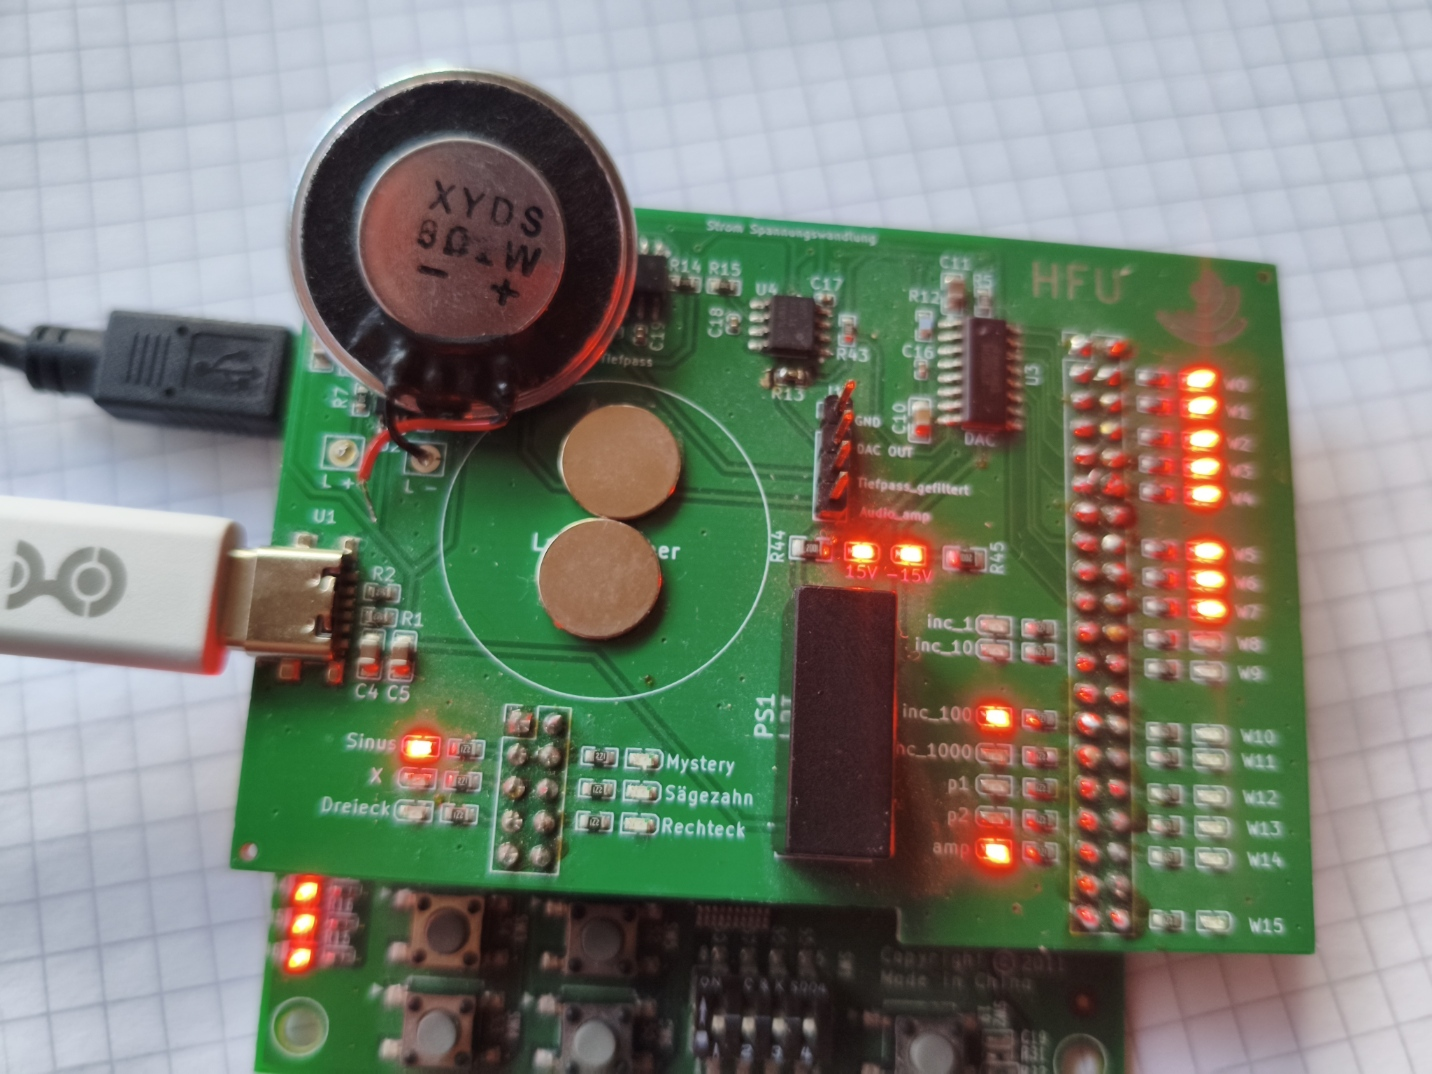
\includegraphics[width=10cm]{img/Lautsprecher-magnet.jpg}
    \caption{Lautsprecher abgenommen, darunter die beiden Magnete zur Befestigung}
    \label{fig:lautsprecher-magnet}
\end{figure}

\section{Stromversorgung und Anschluss}

Für den Betrieb werden zwei USB-Kabel benötigt, die beide angeschlossen sein müssen:

\begin{itemize}
    \item \textbf{USB Mini-B} (am FPGA-Board): wird mit dem Computer verbunden. Dieser Anschluss versorgt das FPGA-Board mit Strom und wird außerdem zum Programmieren des FPGA verwendet.
    \item \textbf{USB-C} (oben auf der Erweiterungsplatine): versorgt ausschließlich die Erweiterungsplatine mit Strom.
\end{itemize}

Ob die Spannungsversorgung der Erweiterungsplatine korrekt funktioniert, lässt sich direkt an den beiden LEDs mit der Beschriftung \texttt{+15V} und \texttt{-15V} ablesen. Leuchten beide, liegt die Versorgungsspannung an und die Platine ist betriebsbereit.

\begin{figure}[H]
    \centering
    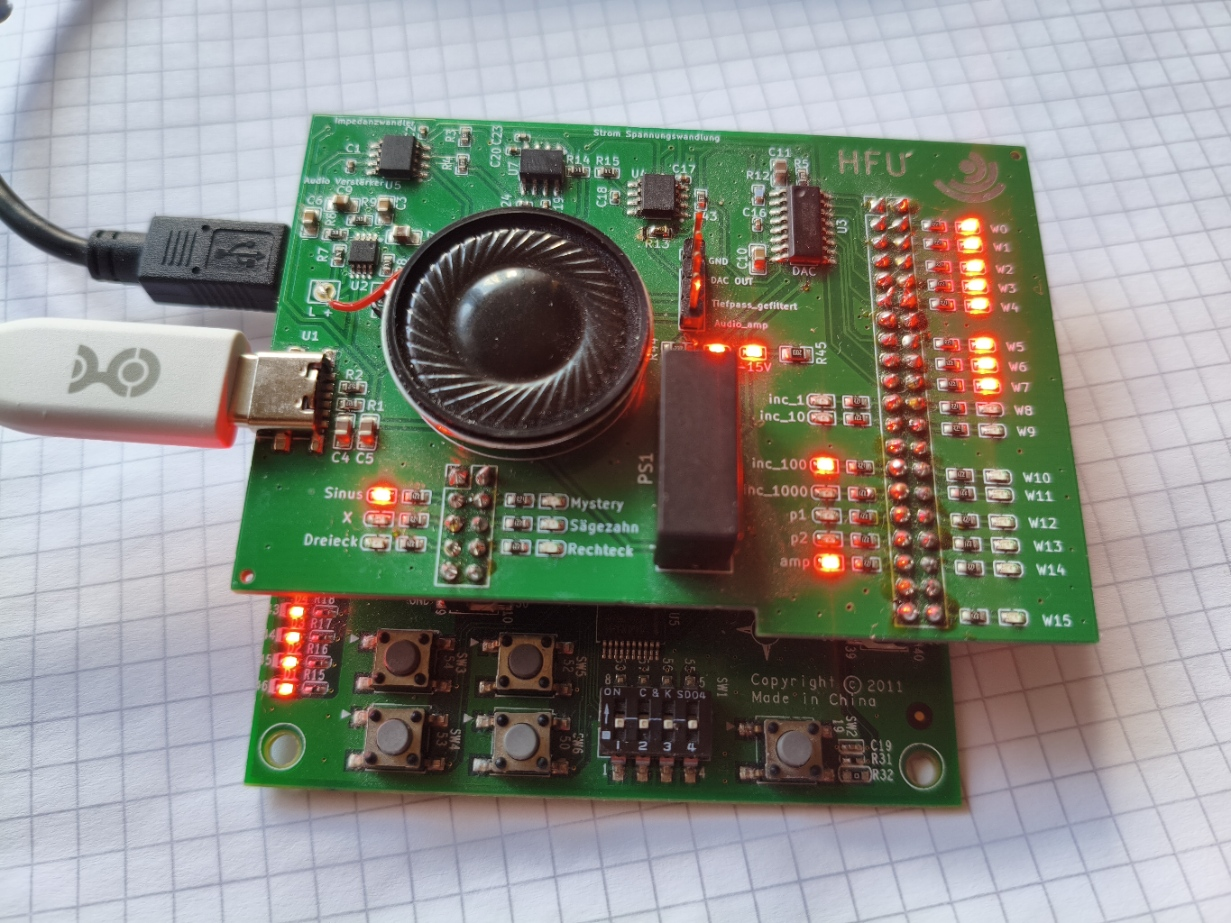
\includegraphics[width=10cm]{img/Signalgenerator_angesteck.jpg}
    \caption{Aufgestecktes Board mit angeschlossenem USB Mini-B, die LED \texttt{-15V} zeigt eine korrekte Spannungsversorgung an}
    \label{fig:board-connected}
\end{figure}

\section{Signalabnahme}

Zur Abnahme der Signale, etwa zum Anschließen eines Oszilloskops, befindet sich auf der Erweiterungsplatine eine Stiftleiste mit den Beschriftungen \texttt{GND}, \texttt{DAC OUT}, \texttt{Tiefpass gefiltert} und \texttt{Audio\_amp}. Zum Abgreifen der einzelnen Signale werden Steckerleisten-Kabel (Jumper-Kabel) verwendet, die einfach auf die entsprechenden Stifte aufgesteckt werden, wie in Abbildung~\ref{fig:signalabnahme} zu sehen.

\begin{figure}[H]
    \centering
    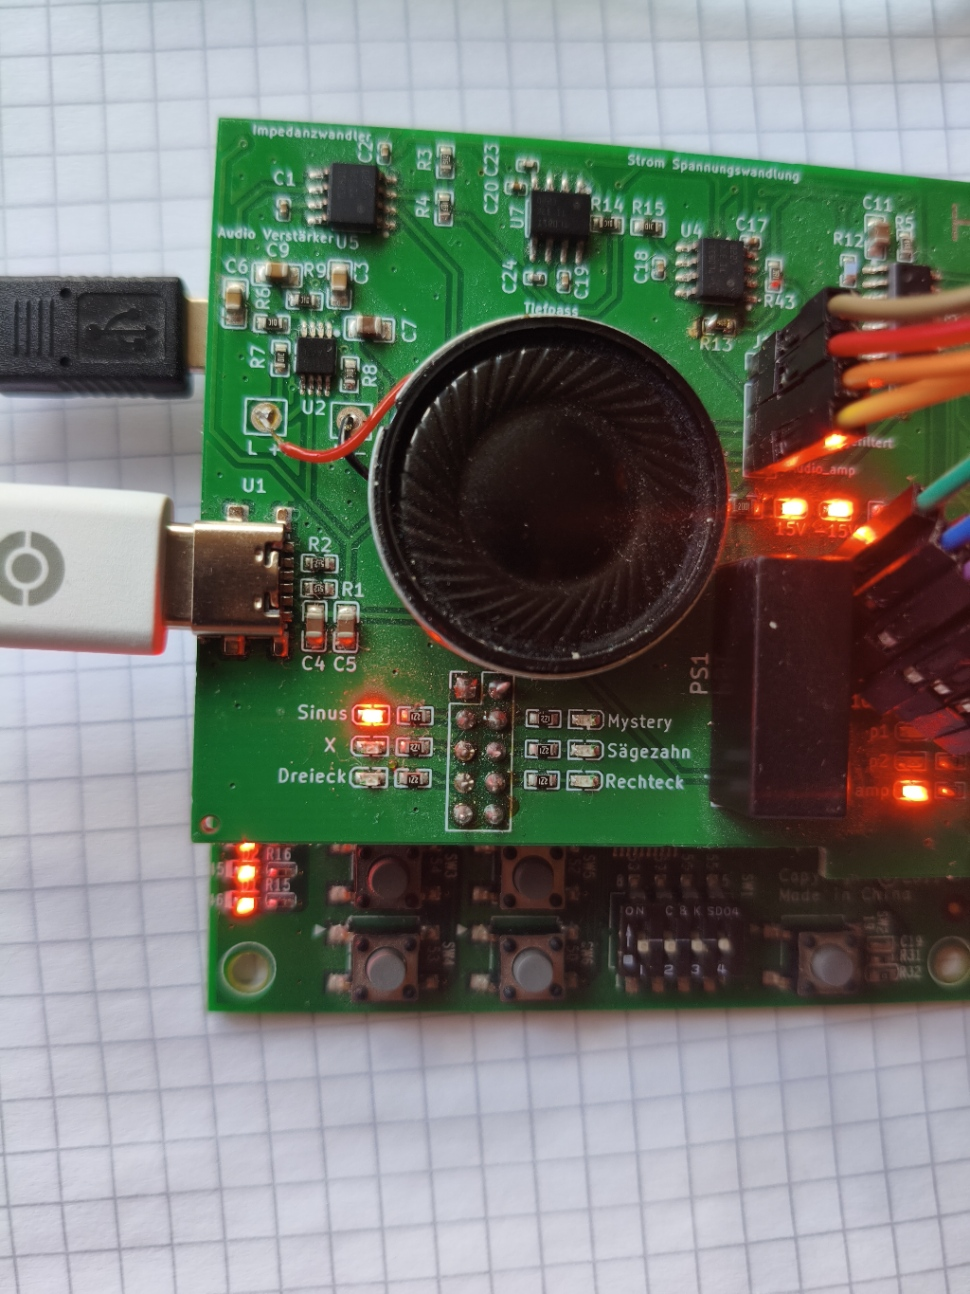
\includegraphics[width=10cm]{img/fertig_monitiert_mit_stecker.jpg}
    \caption{Signalabnahme über Steckerleisten-Kabel an der Stiftleiste}
    \label{fig:signalabnahme}
\end{figure}

Um nachzuvollziehen, welche Station das Signal zwischen diesen vier Abgriffpunkten durchläuft, lohnt sich ein Blick in den beigefügten Schaltplan im Anhang. Er zeigt den vollständigen Signalpfad vom DAC-Ausgang über Tiefpassfilter und Audioverstärker bis zum Lautsprecher.

\section{Anzeige LEDs}
Um dir jederzeit mitzuteilen, was der Signalgenerator gerade tut, sind auf der
Erweiterungsplatine mehrere LED Gruppen verteilt. Jede Gruppe hat eine eigene
Funktion und zeigt dir einen bestimmten Zustand des Systems an.
\begin{figure}[H]
    \centering
    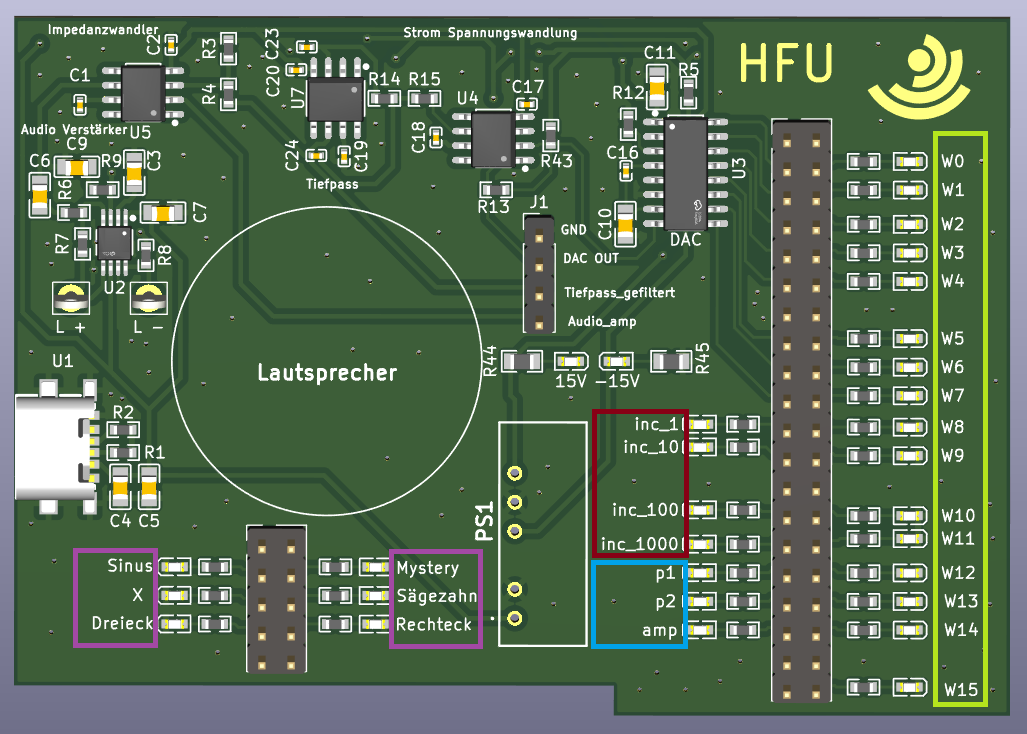
\includegraphics[width=15cm]{img/Platine_1.png}
    \caption{Signalgenerator Platine}
    \label{fig:pcb-board}
\end{figure}

\begin{itemize}
    \item \textbf{Aktueller Parameterwert (grün)}  
    Rechts im Bild befindet sich eine vertikale Reihe (grün) LEDs.  
    Sie zeigen den \emph{numerischen Wert} des aktuell ausgewählten Parameters
    (Amplitude, P1 oder P2) in binärer Form an.  
    Wenn du also z.\,B. die Amplitude veränderst, kannst du hier direkt sehen,
    welchen Wert sie gerade hat.

    \item \textbf{Aktiver Parameter (blau)}  
    Die blau markierten LEDs zeigen dir, \emph{welcher Parameter} momentan
    ausgewählt ist. Immer genau eine der drei LEDs leuchtet:
    \begin{itemize}
        \item LED 0: P1 (Feinfrequenz)
        \item LED 1: P2 (Taktteiler)
        \item LED 2: Amplitude
    \end{itemize}

    \item \textbf{Schrittweite / Increment (rot)}
    Die rot markierten LEDs zeigen an, um welchen Betrag der aktuelle Parameter
    bei jedem Tastendruck erhöht oder verringert wird. Auch hier leuchtet immer
    genau eine LED, die zugehörige Schrittweite steht direkt daneben auf der
    Platine aufgedruckt.
    Diese Anzeige ist besonders hilfreich, wenn du schnell große Werte ändern
    möchtest.

    \item \textbf{Aktive Wellenform (lila)}  
    Die lila markierten LEDs zeigen dir, welche Wellenform aktuell ausgegeben
    wird. Auch hier leuchtet immer genau eine LED, in der Anordnung aus
    Abbildung~\ref{fig:pcb-board}:
    \begin{itemize}
        \item Sinus
        \item X (deine Funktion)
        \item Dreieck
        \item Mystery
        \item Sägezahn
        \item Rechteck
    \end{itemize}
\end{itemize}

Alle LEDs aktualisieren sich in Echtzeit und geben dir damit eine direkte
Rückmeldung über den Zustand des Systems und die Wirkung deiner Eingaben.


\section{Bedienung}
Die in Abbildung~\ref{fig:ui-skizze} dargestellten Tasten bilden die komplette
Benutzeroberfläche des digitalen Signalgenerators. Über fünf Taster können
Wellenform, Parameter und Parameterwerte direkt am FPGA eingestellt werden.

\begin{figure}[H]
    \centering
    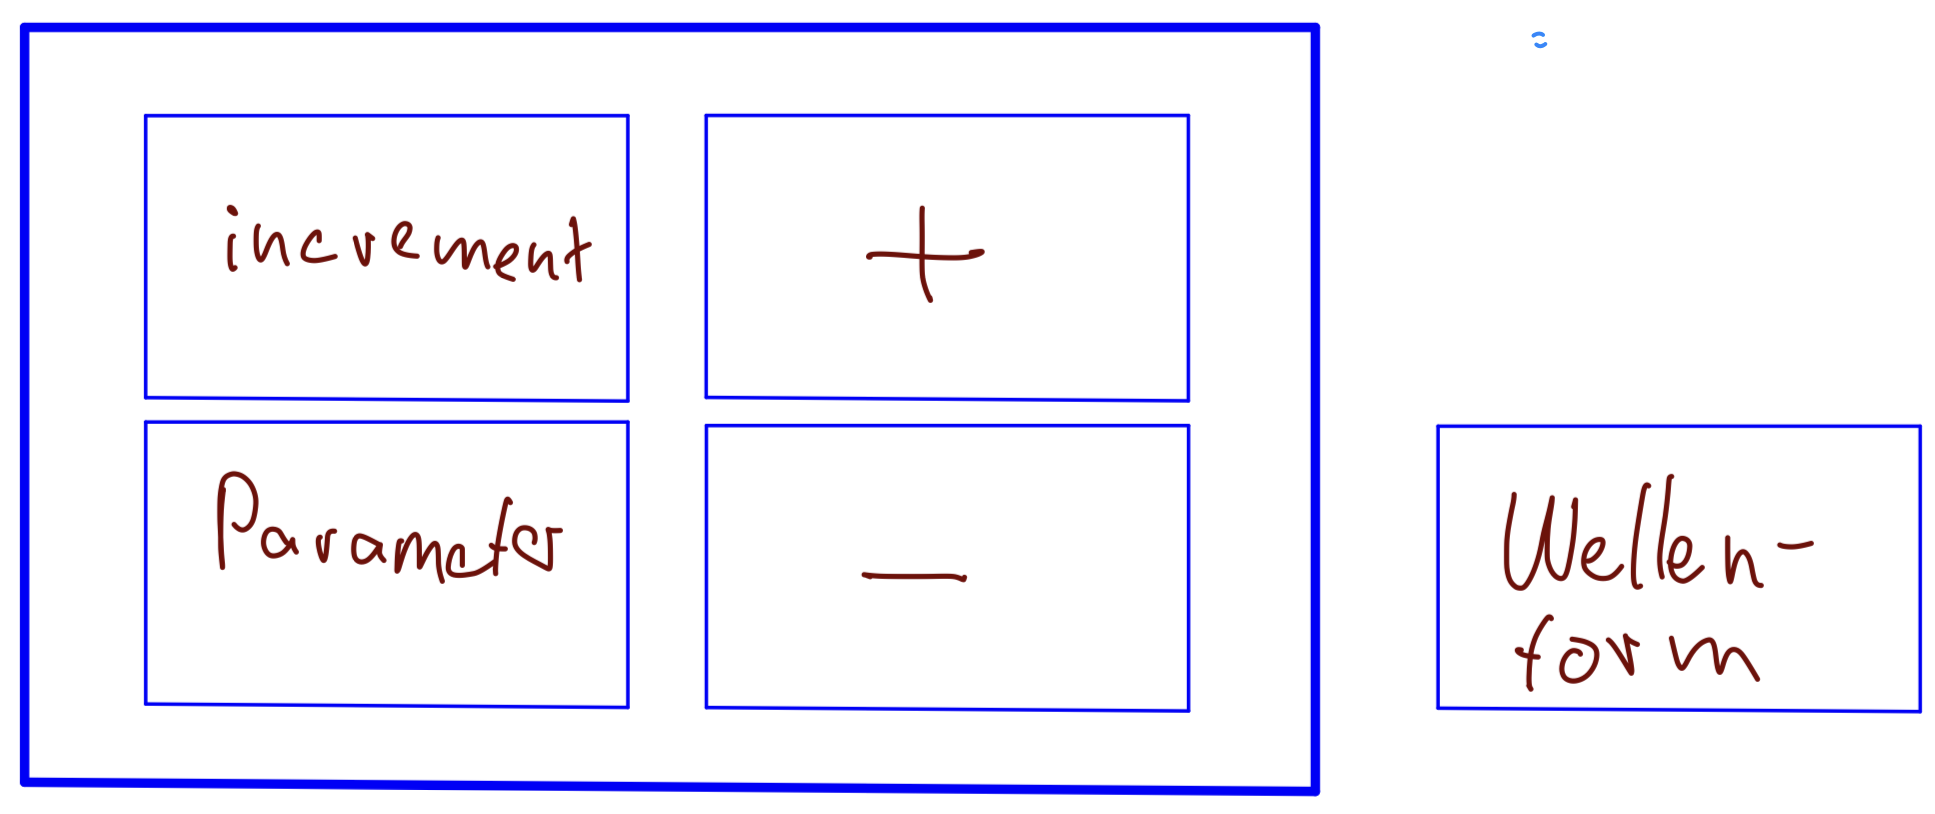
\includegraphics[width=10cm]{img/steuerungs_bottonbelegung.png}
    \caption{Skizze Tastenbelegung}
    \label{fig:ui-skizze}
\end{figure}

Vier der fünf Taster sind als Block gruppiert: \texttt{btn\_param} (SW3) unten
links, \texttt{btn\_inc} (SW4) oben links, \texttt{btn\_plus} (SW5) oben
rechts und \texttt{btn\_minus} (SW6) unten rechts. Der Taster zur
Wellenformauswahl, \texttt{btn\_mode} (SW2), sitzt separat davon.

\begin{itemize}
    \item \texttt{btn\_mode}  (SW2)
    \item \texttt{btn\_param} (SW3)
    \item \texttt{btn\_inc}   (SW4)
    \item \texttt{btn\_plus}  (SW5)
    \item \texttt{btn\_minus} (SW6)
\end{itemize}

Im Folgenden sind alle Tasten und ihre Funktion detailliert beschrieben.

\subsection*{Tastenbeschreibung}

\begin{itemize}
    \item \textbf{SW2 – Wellenform umschalten (\texttt{btn\_mode})}  
    Durch jeden Tastendruck wird zur nächsten Wellenform weitergeschaltet.
    Die Reihenfolge entspricht der LED-Codierung:
    \begin{itemize}
        \item Sinus
        \item X (Reserve)
        \item Dreieck
        \item Mystery
        \item Sägezahn
        \item Rechteck
    \end{itemize}
    Die aktuell aktive Wellenform wird über \texttt{led\_Modus} angezeigt.

    \item \textbf{SW3 – Parameterwahl (\texttt{btn\_param})}  
    Mit diesem Taster wählst du aus, welcher Parameter verändert werden soll.
    Die Auswahl läuft zyklisch durch:
    \begin{itemize}
        \item \textbf{P1} – Feinfrequenz / DDS-Inkrement
        \item \textbf{P2} – globaler Taktteiler
        \item \textbf{AMP} – Amplitude (0–255)
    \end{itemize}
    Der aktive Parameter wird über \texttt{led\_param} (1‑Hot) angezeigt.

    \item \textbf{SW4 – Schrittweite umschalten (\texttt{btn\_inc})}  
    Dieser Taster bestimmt, wie stark ein Parameter pro Tastendruck verändert wird.
    Die Schrittweiten sind:
    \begin{itemize}
        \item 1
        \item 10
        \item 100
        \item 1000
    \end{itemize}
    Die aktive Schrittweite wird über \texttt{led\_inc} angezeigt.

    \item \textbf{SW5 – Wert erhöhen (\texttt{btn\_plus})}  
    Erhöht den aktuell ausgewählten Parameter um die eingestellte Schrittweite.
    Der neue Wert wird binär über \texttt{led\_W} ausgegeben.

    \item \textbf{SW6 – Wert verringern (\texttt{btn\_minus})}  
    Verringert den aktuell ausgewählten Parameter um die eingestellte Schrittweite.
    Auch hier zeigt \texttt{led\_W} den aktuellen Wert an.
\end{itemize}

\subsection*{Zusammenspiel der Bedienung}

Die Bedienung folgt einem einfachen Prinzip:
\begin{enumerate}
    \item \textbf{Mit SW3 wählst du den Parameter} (P1, P2 oder AMP).
    \item \textbf{Mit SW4 stellst du die Schrittweite ein} (1, 10, 100, 1000).
    \item \textbf{Mit SW5 und SW6 erhöhst oder verringerst du den Wert}.
    \item \textbf{Mit SW2 wechselst du die Wellenform}.
\end{enumerate}

Alle Änderungen wirken sich sofort auf das Ausgangssignal \texttt{analog\_out}
aus, das über den DAC ausgegeben und am Oszilloskop sichtbar wird.
